\documentclass[
  11pt, % The default document font size, options: 10pt, 11pt, 12pt
  codirector, % Uncomment to add a codirector to the title page
]{charter}
\usepackage{enumitem}
\usepackage{pdflscape}
\usepackage{tikz}
%\usetikzlibrary{shapes,arrows}
%\usepackage{tikz}
\usetikzlibrary{positioning, arrows.meta, backgrounds, fit}
\usepackage{fontawesome5}
\usepackage{tikz,tkz-tab}
\usepackage{booktabs} % Para tablas más elegantes
\usetikzlibrary{positioning, arrows.meta, backgrounds, fit}

\usetikzlibrary{matrix,arrows, positioning,shadows,shadings,backgrounds, calc, shapes, tikzmark}

\usepackage{fmtcount}
\usepackage{xurl}



% Completar los siguintes Campos
\materia{Testing de Software en Sistemas Embebidos}
\bimestre{cuarto bimestre}
\docentes{Alejandro Permingeat; Esteban	Volentini; Mariano Finochietto y Rafael Oliva}
\titulo{Testing de emulador de microprocesaro Leon3 para desarrollo de software satelital y simuladores}
\posgrado{Carrera de Especialización en Sistemas Embebidos}
\autor{Ing. Iriarte Fernandez, Nicolás Ezequiel
  (NicolasIriarte95@gmail.com)}
\director{Esp. Lic. Horro, Nicolás Eduardo}
\pertenenciaDirector{INVAP.\@S.E.}
\codirector{}
\pertenenciaCoDirector{}
\fechaINICIO{11 de Abril de 2024}

\begin{document}

\maketitle
\tableofcontents

\newpage

\section*{Registros de cambios}
\label{sec:registro}


\begin{table}[ht]
	\label{tab:registro}
	\centering
	\begin{tabularx}{\linewidth}{@{}|c|X|c|@{}}
		\hline
		\rowcolor[HTML]{C0C0C0}
		Revisión & \multicolumn{1}{c|}{\cellcolor[HTML]{C0C0C0}Detalles de los cambios realizados} & Fecha      \\ \hline
		0      & Creación del documento.                                 &\fechaInicioName \\ \hline



    \hline

	\end{tabularx}
	\label{sec:cierre}
\end{table}

%% \pagebreak


\section*{Documentos anexos}
\label{sec:documentos_anexos}

%%%%%%%%%%%%%%%%%%%%%%%%%%%%%%%%%%%%%%%%%%%%%%%%%%
\begin{table}[h!]
	\centering
	\begin{tabular}{ | m{1.5cm} | m{3cm} | m{10.5cm} | }
		\hline
		\rowcolor{gray!50} % Coloring the first row
		\textbf{Ref.} & \textbf{Nombre} & \textbf{Descripción} \\ \hline
    AD.01 & NEMU-SRD-1 & Especificación de requerimientos de software. \\ \hline
		AD.02 & NEMU-UCD-0 & Defenición de casos de uso y arquitectura de software. \\ \hline
		AD.03 & NEMU-MTP-0 & Master Test Plan.\\ \hline

	\end{tabular}
  \caption{Documentos anexos.}
  \label{tab:referencias}

\end{table}
%%%%%%%%%%%%%%%%%%%%%%%%%%%%%%%%%%%%%%%%%%%%%%%%%%

\pagebreak


\section{Introducción}
\label{sec:org60390fa}

En el presente documento se detallarán once ensayos a nivel sistema de aceptación del componente de software ``CPU'', perteneceinte al emulador de microprocesador Leon3. El objetivo de estos ensayos es verificar que el componente cumple con los requerimientos de software especificados en el documento \textbf{NEMU-SRD-1}.

Previo a dicho documento, se recomiendo la lectura del documento ``Master Test Plan'', anexado en la tabla de referencias del presente documento como \textbf{NEMU-MTP-0}.


\section{Diseño de casos de prueba}
\label{sec:org12376an}

A continuación se detallan los casos de prueba a nivel sistema que se realizarán sobre el componente de software ``CPU'', respecto a ciertos requerimientos especificos que se complementan en conjunto para un caso de uso.

Requerimientos a testear:

\begin{itemize}
\item \textbf{NEMU-SR-01}: El software deberá proveer acceso a los registros del procesador emulado.
\item \textbf{NEMU-SR-03}: El software deberá poder cargar los mismo binarios que el microprocesador fisico.
\item \textbf{NEMU-SR-06}: El software deberá emular las instrucciones de lectura y escritura de memoria.
\item \textbf{NEMU-SR-07}: El software deberá emular las instrucciones de suna, resta y multiplicación.
\item \textbf{NEMU-SR-08}: El software deberá emular las instrucciones de salto condicionales, tales como operadores \textit{if} y \textit{jumps}.
\end{itemize}

Para el desarrollo de los ensayos, se emplea la técnica de diseño de ``Classification-Tree method'' \textbf{CTM}, la cual se compone de los pasos:
\begin{enumerate}
\item Identificación de los aspectos bajo prueba.
\item División del dominio de entrada de acierdo con los aspectos.
\item Especificación de los casos de prueba lógicos.
\end{enumerate}


Mediante esta técnica, se logra una cobertura de los casos de prueba de manera eficiente y efectiva. Generando la cantidad mínima de casos de prueba necesarios para cubrir el dominio de entrada.

\newpage

\begin{figure}[htpb]
  \label{fig:CTM}
  \centering
  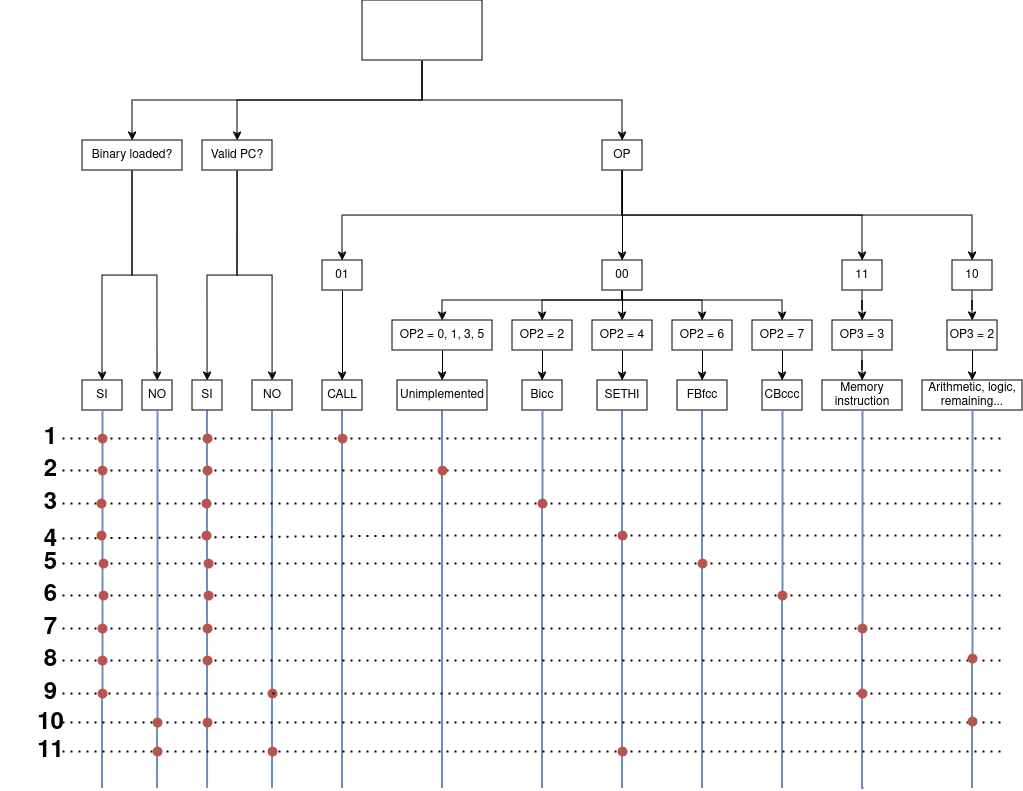
\includegraphics[width=1\textwidth]{./Figuras/CTM.png}
  \caption{Diagrama CTM.}
\end{figure}

\vspace{25px}

\textbf{NOTA}: Debido a la extensa cantidad de intrucciones disponibles para el procesador seleccionado, el arbol fué acotado y/o simplificado para toman unicamente las instrucciones más representativas y variadas, no siendo la totalidad de las instrucciones disponibles.


Dada la Figura \ref{fig:CTM}, se procede a la generación de los casos de prueba lógicos, los cuales se detallan en la siguiente tabla:

%%%%%%%%%%%%%%%%%%%%%%%%%%%%%%%%%%%%%%%%%%%%%%%%%%
\begin{table}[h!]
	\centering
	\begin{tabular}{ | m{2cm} | m{5cm} | m{7cm} | }
		\hline
		\rowcolor{gray!50} % Coloring the first row
		\textbf{CASO} & \textbf{ASPECTO} & \textbf{RESULTADO ESPERADO} \\ \hline
    1 & Binario cargado \newline
        PC valido \newline
        OP: 01 \newline
      & Ejecución exitosa \\ \hline

    2 & Binario cargado \newline
        PC valido \newline
        OP: 00 \newline
        OP2: 01 \newline
      & Error, instrucción invalida \\ \hline

    3 & Binario cargado \newline
        PC valido \newline
        OP: 00 \newline
        OP2: 02 \newline
      & Ejecución de instrucción Bicc exitosa \\ \hline

    4 & Binario cargado \newline
        PC valido \newline
        OP: 00 \newline
        OP2: 04 \newline
      & Ejecución de instrucción SETHI exitosa \\ \hline

    5 & Binario cargado \newline
        PC valido \newline
        OP: 00 \newline
        OP2: 06 \newline
      & Ejecución de instrucción FBfcc exitosa \\ \hline

    6 & Binario cargado \newline
        PC valido \newline
        OP: 00 \newline
        OP2: 07 \newline
      & Ejecución de instrucción CBccc exitosa \\ \hline


	\end{tabular}

  \newpage

\end{table}


\begin{table}[h!]
	\centering
	\begin{tabular}{ | m{2cm} | m{5cm} | m{7cm} | }
		\hline
		\rowcolor{gray!50} % Coloring the first row
		\textbf{CASO} & \textbf{ASPECTO} & \textbf{RESULTADO ESPERADO} \\ \hline


    7 & Binario cargado \newline
        PC valido \newline
        OP: 11 \newline
        OP3: 03 \newline
      & Ejecución de instrucción exitosa \\ \hline

    8 & Binario cargado \newline
        PC valido \newline
        OP: 10 \newline
        OP3: 02 \newline
      & Ejecución de instrucción exitosa \\ \hline


    9 & Binario cargado \newline
        PC invalido \newline
        OP: 11 \newline
        OP3: 03 \newline
      & Error, PC invalido \\ \hline

   10 & Binario no cargado \newline
        PC valido \newline
        OP: 10 \newline
        OP3: 02 \newline
      & Error, binario no cargado \\ \hline

   11 & Binario no cargado \newline
        PC invalido \newline
        OP: 00 \newline
        OP2: 04 \newline
      & Error, binario no cargado \\ \hline



	\end{tabular}

\end{table}
%%%%%%%%%%%%%%%%%%%%%%%%%%%%%%%%%%%%%%%%%%%%%%%%%%


\end{document}
